\documentclass [11pt,a4paper]{article}
\usepackage[margin=1.2in]{geometry}
\usepackage{graphicx, lscape, url}
\usepackage{wrapfig}
\usepackage{float}
\usepackage{textcomp, gensymb}
\usepackage{subfig}

\setlength
\parindent{0pt}

\begin{document}
 
% Titlepage
\thispagestyle{empty}
\begin{center}
    \centering
% University logo
    
\includegraphics[width=0.3\linewidth]{images/nottingham-logo.png}
    \vspace{0.1cm}
    {\Large \\University of Nottingham\par}
    {\Large Department of Computer Science\par}
    \vspace{3cm}
% Project title
    {\Large COMP3003 - Interim Report\par}
    \vspace{0.5cm}
    {\Large A Cross-platform Networking Configuration \& Auditing Mobile Application\par}
    \vspace{2.5cm}
% Author Name
    {\Large Jozef W. Sieniawski\par}
    {\small Computer Science BSc. \par}
    {\small 20296126 $|$ psyjs25@nottingham.ac.uk\par}
    \vspace{1cm}
% Supervisor
    {\normalsize Supervisor: Prof. Chris Greenhalgh\par}
    \vspace{3cm}
% Date
    {\Large December 2022}
\end{center}

\pagebreak
\pagenumbering{roman}    

\begin{abstract}
    \noindent
    For Small/Medium, and even some large companies that own and maintain their own server spaces, a unique set of challenges are to be faced. Although these devices are typically business critical, they are typically squeezed into encumbered spaces, with lacklustre lighting and limited access. Further, and critically, this makes the maintaining and documenting of these devices inherently more difficulty. Current alternative solutions fail to focus on in-situ use, and are typically bloated with features for large data centers. This project investigates the needs and requirements that can solves these challenges, with a focus on Human-Computer Interaction. From these designs, this project then implements a cross-platform mobile application that satisfies these needs.

\end{abstract}

% Table of contents
\pagebreak

\tableofcontents
\pagebreak 
\pagenumbering{arabic}    

% Add spacing between paragraphs
\setlength{\parskip}{2ex}

% Introduction
\section{Introduction}
\label{sec:introduction}
With the work for the Research Support Team in the School of Computer Science at Nottingham, one of the primary responsibilities revolves around server spaces. This involves the installation and configuration of new servers, as well as the maintenance of existing hardware. When we were faced with the task of migrating servers to a new location, the problem of understanding the configuration of the existing servers arose. There lacked a consistent documentation format that could be used to replicate the configuration of a server in a new location.

With a larger project in mind, where understanding the configuration of many servers was essential, the idea of this project was born; To create a tool that will allow for cable configuration of server hardware to be easily digitised, visualised, queried and updated.

Whilst alternatives exist, they are typically a segment of a far larger suite of tools, which are usually not necessary for small/medium sized server spaces. Naturally, cable configurations can be difficult to understand and work with even in these smaller spaces. This also brought forward the second aspect of the project, to also be an investigation into the user experience and interface design of the tool. To ensure that the tool is easy to use and can be understood by a wide range of users.

Further, the project will be open source, and will be available for use by the wider community of server administrators. This will allow for the human Computer interaction findings that have been implemented to be used in similar applications. Additionally, the tool will be utilising and integrating with Netbox\cite{Netbox}, an open-source tool for managing network infrastructure. This will act as the backing database for the tool and will allow for the tool to be used in a wider context of server management.

The Research Support Team will act as a prime example of the target audience. The project aims to discover the needs of a wider range of small and medium sized enterprises (SME) who run and maintain their own server spaces. As mentioned previously, there are not many similar alternatives to the project as these SME's usually pose a unique server environment. These spaces can be cramped, poorly lit and hard to navigate. Seen below is a picture of the server space in the School of Computer Science at Nottingham (fig. 1), which is an example of the type of environment that the project will be designed for.
\begin{figure}[H]
    \centering
    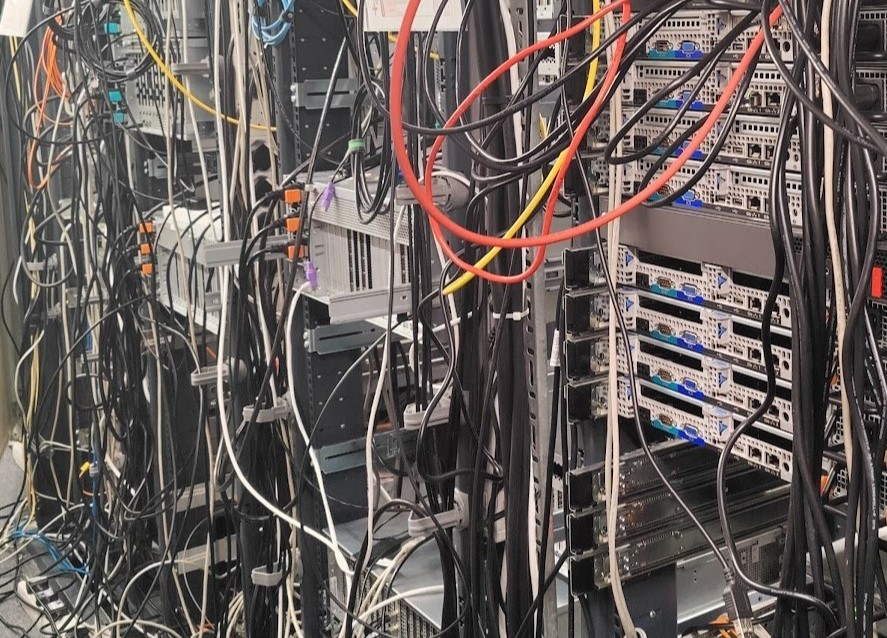
\includegraphics[width=0.55\linewidth]{images/server_racks.jpg}
    \caption{Server Rack within the school of Computer Science}
    \label{fig:server_rack}
\end{figure}

This is another reason that typical solutions cannot usually apply to these spaces, as they are often designed for large data centres, where laptops can be used easily to use software in situ. A tool that can be used on a mobile device in these less-than-ideal conditions is something worthy of investigation. As mentioned, a perfect example of this is the server space in the School of Computer Science seen a (Fig. \ref{fig:server_rack}). Before upgrades, the space was poorly lit and is, still relatively cramped. It’s not particularly feasible to use a laptop in this space comfortably, which most solutions rely on due to cluttered UI. The current layout of servers and hardware makes tracking cables completely impracticable and a mobile application would be a perfect solution to this problem. 

\begin{figure}[H]
    \centering
    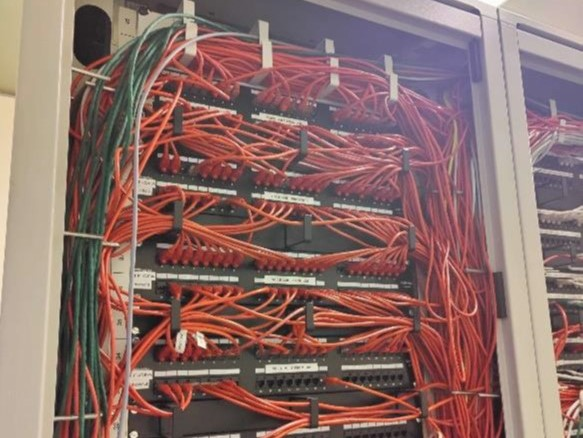
\includegraphics[width=0.55\linewidth]{images/server_racks_clean.jpg}
    \caption{More ideal and realistic server space}
    \label{fig:ideal_server_space}
\end{figure}

\pagebreak
Comparatively, the server space dedicated to networking has been managed to a more ideal state (fig. \ref{fig:ideal_server_space}). Whilst not perfect, comparing to that of data centers, it is far more manageable. This is the aim of the project, to create a tool that can be used in these less-than-ideal conditions to allow for scenarios like the one in fig. \ref{fig:server_rack} to be managed more easily.

\subsection{Aims \& Objectives}
\label{sec:objectives}
The projects aims with their respective objectives.
\begin{enumerate} 
    

    \item[A1] To create a tool that will allow for cable configuration of server hardware to be
    easily digitised, visualised, queried and updated. 
        
        - In order to achieve this, the tool will integrate with Netbox, an open-source tool for managing network infrastructure. This will act as the backing database for the tool and will allow for the tool to be used in a wider context of server management.
        
        - The tool will use Netbox's API to query and update the database whilst using intuitive UI to allow for easy use.
        
        - To achieve visualisations, the tool will illustrate the cable connections between devices, showing data in a clear and concise manner.

    \item[A2] To create a in situ cross platform mobile app that can be utilised in restricted
    spaces.    

        - To achieve this, the tool will be cross platform, and will be able to be used on any mobile device supported by the Flutter framework.
        
        - The tool will be designed with a focus on Human-Computer Interaction, to ensure that the tool is easy to use and can be understood by a wide range of users.

    \item[A3] To create an app that can interact with other open-source software easily
    
        - The tool will be open source, and so modifications can be made to the tool to allow for it to be used in other contexts.
        
        - The tool will be built around modifiable models that can be changed easily for other software or a custom build backend.

\end{enumerate}
\pagebreak
\subsection{Background}
\label{sec:background}

There are currently no popular mobile tools for this use case. Whilst I can appreciate, in a large data centre application. It is likely that a mobile application might not have the same level of functionality as a desktop application. Further, it is likely to be useful in a larger environment. But with my experiences working for the Research Support Team - I have personally found that a tool of this nature would be extremely useful. Further, with the Open Source nature of Netbox, the accepted DCIM software for RST, a mobile application would be a perfect companion. With the addition that the tool could then be released to the wider community of server administrators to be used with their own instances of Netbox.

\section{Related Work}
\subsection{Application and Product Reviews}
\label{sec:app_reviews}

Following research of open source and paid for cable management/DCIM software I have found that there are limited options that allow for trial version without a legitimate business interest. This limited the selection of software that can be researched. There follows three different software packages that I have found that are relevant to the project. Including Sunbird DCIM\cite{Sunbird}, a paid for solution with a trial accessible publicly. Pathfinder Mobile \cite{Pathfinder}, a mobile counterpart to the enterprise "Pathfinder" package, this was the only high quality mobile solution that was discovered. Finally, Netbox \cite{Netbox}, the open source DCIM software that the project will be built around. These three packages were shown to three individuals within the Research Support Team and their feedback was recorded. Each software was shown in mobile view. 

\subsubsection{Sunbird DCIM}
\label{sec:sunbird}
Sunbird DCIM is a feature full Data Centre Infrastructure Management Package with a significant list of components. Their client list includes the Paddypower betfair, ebay and COMCAST \cite{Sunbird-we-know-data-centres}. When trialling dcTrack their DCIM software - The immediate impression is that it is feature-rich; including Environment, Security, Cooling as well as Asset and Connectivity. Whilst the server spaces within Computer science at UoN could benefit from a tool like this. 
Its implementation and management would be strenuous. The tool is designed for large data centres and would be overkill for the server spaces within the school. But, some of its features could be useful in the implementation of the project. For example, the visualisation of data centers via a 3D model. This could be an interesting feature to implement in the project but might be out of scope. The searching of assets and connections, while thorough, is not as intuitive as the project aims to be. Further, the intention of Sunbird is to serve clients that might have thousands of assets, not quite hundreds. So the requirements of searching and filtering are different. Though, filtering by an extensive set of categories is a useful feature and could be implemented in the project, but in a more intuitive manner. 

\subsubsection{Pathfinder Mobile}
\label{sec:pathfinder}
Pathfinder Mobile is a mobile component to the complete Pathfinder package. The mobile application is designed to be used in conjunction with the full software and used as an "anytime and anywhere" tool. It allows existing users of Pathfinder to access data remotely and in-situ. With a intriguing focus on, "work orders". Being created at a workstation, i.e. Laptop, then the mobile app synchronizes with these work order. Then the mobile app can be used to execute these work orders on site through using "graphical instructions support"\cite{Pathfinder}. Finally, then, all changes are uploaded to the pathfinder client. A similar environment interaction would work well for this project. With more complex modifications being completed/generated on a desktop client on the Schools Netbox instance, i.e Templating. Then once completed, the data entry for these templates can be completed on the mobile app, in the server space. With the app synchronising with Netbox via its API. 

The pathfinder app also allows for quick access to networking information, where users can complete tracing of connections.Whilst this already was a core intention of the project, Pathfinders method to visualise this is intuitive and similar to that which was discussed in the first Current State Analysis interview. These interviews are discussed more in detail in section \ref{sec:current_state_analysis}. But, notably, an interviewee mentioned a good method to do a visualisation is to list devices in a scrollable view - with the connections between them being drawn on the screen, along with device and interface information displayed as well. This is similar to the method used by Pathfinder, with; device name, location, interface name, type and cable type being displayed. 

One aspect of Pathfinder that could be improved upon is the searching of assets. Whilst they describe their searching as being "text-rich" - It seems to be less intuitive, and does a search based on every field, meaning that results for a simple search can be overwhelming. This is something that the project aims to improve upon, with a more intuitive search method. Further, their search by ID code only simply enters the ID code into the search bar. This is not a bad method, but it is not as intuitive as it could be. 

Overall, I think pathfinders mobile app will be a good reference point for the project. It has a similar focus to the project, and has a similar method of visualising data. Though it is a companion of a larger software package that doesn't meet the requirements of the school, it has features that can be referred to and implemented in the project.

\subsubsection{Netbox}
\label{sec:netbox}
Whilst searching for a DCIM solution for the School of Computer Science - Netbox become a clear choice. It has a great feature core, it's open source, self-'hostable' and is able to help solve the problems that the school is facing. As discovered during the Current State Analysis and my own experiences, the server rooms within CS are poorly documented due to a lack of consistent historical data. Most of the information is stored in memory of long gone staff, or in out of date spreadsheets. Netbox is to act as a "source of truth"\cite{Netbox}. 

It has become the accepted DCIM solution for the Research Support Team and will be a key aspect to this project. Though, it does have some limitations, the most notable being a lack of visualisations, and the entry and querying of cable management data. This is where the project will come in as a supporting tool. 

\subsection{Papers focused on HCI and User Experience}
\label{sec:HCI}
There is a lack of significant research into areas of Human-Computer Interaction and User Experience in the context of server management. But there are a few papers that are relevant to the project. The first paper is a write-up by Yin et al. \cite{cloud3dview} regarding their demonstration of Cloud3DView at SIGCOMM '13. Cloud3DView is an interactive 3D visualisation tool used for Data Centers which uses FPS gamification to allow users to monitor situations and control data from a user friendly interface. This project also included a focus on "cutting-edge HCI technologies" \cite{cloud3dview}. Whilst the paper itself doesn't go into reasoning of why certain HCI choices were made - It shows a good example of how a mobile device can be used to interact with a data centre, and can be used to improve efficiency and user experience. Whilst the focus of this project isn't to be a 3D visualisation tool, one aspect of Cloud3DView is the ability to view data in relation to the devices in a 3D environment. Whilst, a 3D visualisation is out of scope for KeepTrack - It is possible that an augmented reality view could be implemented, where users can view data/connections in relation to the devices via a camera on their mobile device. In fact, this was a feature suggested by an interviewee during the Current State Analysis.

Further, there was a focus on using mobile devices to be used for the visualisation, but didn't mention the use of a mobile device for data entry. With the nature of the data being entered in the context of data centers, a mobile format will be more intuitive/accessible than a desktop format for some cases. An important benefit of using mobile devices for data entry is a the ability to use multiple interface types to enter data. For example, a user can enter data via an alphanumeric keyboard, numerical keypad, calendar picker, lists etc. A comparative analysis into different data entry design patterns investigated 3 different patterns for 7 different data types for a set of 9 tasks testing different patterns \cite{myka2019comparative}. For this project, the most relevant data types are; dates, small numbers, single-choice lists and text. The investigation completed a set of usability tests to determine which pattern was the most effective, with different patterns benefiting different tasks/data types better than others. The results from this study will be used to inform the design of the interface for the project, and will be discussed in more detail in section \ref{sec:design}. 

On a similar note, a study into the structure of data entry on mobile devices noted that existing interfaces "interfere with user input" and force "complex interactions to enter simple information" \cite{van2007gui}. This is especially apparent in some cases of the netbox interface. Whilst, naturally, there are limitations as to how simple an interface can be on a desktop based web application, there is more room for improvement on a mobile application. Kleek et als \cite{van2007gui} study also focused on the structure of data entry on mobile devices, its importance, but also the importance of not creating interfaces that deter users from entering data. Highlighting a fine balance between the two. For one of the sources of problems for the school is the lack data ever being entered into anywhere. If the project has an interface that dissuades users or is perceived as too tedious then it will not solve a key problem. This project will take upon the findings of this study to ensure that the interface is intuitive and easy to use. For example, an autocomplete search bar for assets and replacing text fields with scanners or other input methods. 

\subsection{Papers focused on Technical aspects of the project}
\label{sec:technical}

Whilst deciding on a cross platform framework to build this project on, Flutter become the obvious choice. Not only in my previous experiences with it but also as it has become the most popular cross platform framework \cite{JetBrainsFlutter}. Further, with my work in aiding the development of Labmonitor\cite{labmonitor}, I have become familiar with the Code scanning package that will also be used in this project\cite{barcodeScannerPlugin}.

One of the key parts where the project aims to improve is the searchability of assets, i.e. finding the asset desired quickly and accurately through many means. The current method of asset identification is inconsistent with different naming conventions, ID codes, labels, no labels, host name etc. The Centre for the Protection of National infrastructure (CPNI) have a paper on the importance of asset management, specifying that "all organisational assets and systems that are necessary for the delivery of effective operations or are of specific organisational value (e.g. commercially sensitive information), should be identified." \cite{cpni}.

Not only is it important to identify assets whilst they are in use, but also for documenting any changes, journal entries, ownership, location etc.
This project also aims to improve upon this, with a focus on the identification of assets being unified and consistent.

In this project, assets are considered to be both physical hardware, such as servers, switches, KVMs etc. but cabling, such as ethernet, fibre, power etc. In order to identify each of these assets uniquely it was decided that a encoded label would be best. A comparative study into barcodes, QR-codes and RFID systems in the library environment looked into the respective advantages and disadvantages of each \cite{lotlikar2013comparative}. Going by these attributes, it is more sensible to use Barcodes or QR codes for the project. With RFID tags being more expensive, and tag collisions can occur when many are in a close proximity - Like that of a server room. Further, a specialised reader is needed and so another handheld device would need to accompany the app.

Additionally, a paper written on the review of QR codes highlights that, QR codes can store more data in same area, have data redundancy, faster to scan and are "readable from any direction in 360\degree"\cite{mishra2017review}.  Whilst these benefits seem to make it the clear choice over barcodes, QR codes contain data in both dimensions - Whilst this is a benefit in most use cases, it is likely to pose a problem when scanning codes stuck to ethernet cables. Where, barcodes contain data in one dimension which is then repeated vertically, allowing for their placement to be more dynamic, e.g. on a cable. This is clearly shown in figure 3 of the paper \cite{mishra2017review}. So, for this project the use of barcodes for cables, and then QR codes for other assets will be used. Especially with the data needed to be stored for cable information needing to be completely abstract, with a random short number being assigned to each cable. This way it can be entered manually if the scanner fails. On the other hand, with assets, e.g. servers - The data can be more specific, and so a QR code will be used. E.g. can contain a URL that links to the asset in the netbox database.

Whilst an Augmented Reality visualisation feature is dependant on time and the success of other elements - It is still important to consider related work with these features, especially as it could be a feature added on. Whilst already investigating Cloud3DView \cite{cloud3dview}, which uses 3D visualisation, a more apt implementation would be by using the QR codes placed on assets to aid in visualising data via Augmented Reality. This is very similar to the work outlined in the paper, "Applying QR code in augmented reality applications" \cite{applyingQR}. This paper displays how the elements of the QR code can be used to position elements in the AR scene and simultaneously generate information embedded in the QR code. Should this be a feature that can be implemented, it is likely I will follow a similar method as to what Kan et al. set out \cite{applyingQR}. With the existing desire to implement a multi-format code scanner, i.e both barcode and QR, this would be a good addition to the project. Further, there already exists a cross platform plugin for Augmented Reality in Flutter which can be utilised \cite{ar_flutter}.

\section{Description of the Work}
\label{sec:work}
The aim of this project is to create a mobile application that will allow for users to add, view and manage assets and cables in server rooms. With the specific application to Small/Medium enterprises. The application will be built using Flutter, a cross platform framework which will allow for the app to be used on both Android and iOS devices. The application will be built upon Netbox DCIM \cite{Netbox} and their RESTful API \cite{NetboxAPI}. 

The project aims to build upon this API to create a more user friendly and intuitive interface for server administrators to use. With this in mind, a second key aspect is investigating the best interface for the data entry in this context. This will be done by interviewing and observing the system administrators at the school using iterative prototypes of increasing fidelity.

\subsubsection{Project Stretch Goals}
\label{sec:stretchgoals}
Following the interviews during the current state analysis and the investigation of similar work, the further goal to implement a augmented reality visualisation feature is desirable. Allowing for the user to visualise asset information and networking details in a highly interactive way. 
Desirable features that could be implemented dependant on time constraints in priority order: 
\begin{itemize}
\item Journals for assets, allowing for notes to be added to assets, e.g. when a new component is added, or when a component is removed.

\item Auditing of assets, allowing for the user to scan an asset and then be presented with a form to fill out, e.g. the asset is in good condition, or the asset is faulty. 

\item In-App SSH terminal, allowing for the user to connect to a device and run commands, e.g. to check the status of a service.
\end{itemize}

\section{Methodology}
\label{sec:methodology}
With all of the aims and aspects of the projects in mind it was decided to use a a participatory design approach, with iterative prototypes of increasing fidelity. Then, with user evaluation and feedback, the final product will be created. This will be done by following the steps outlined in the following sections.

\subsection{Current State Analysis and Initial Interviews}
\label{sec:current_state_analysis}
To begin with, using my personal experience, knowledge and my own understanding of the requirements, I created a set of low fidelity prototypes - primarily to establish an initial set of features. In order to establish a more in-depth baseline for the project, extending on my existing experiences working for the school, as set of interviews were conducted with the system administrators (RST). Within these interviews, the current state of the system was discussed, with the aim of understanding the current workflow and the problems that are faced. This was done by asking broad questions such as:

\begin{itemize}
    \item What are your opinions on the current state of the server room?
    \item What do you think could be improved?
    \item Do you have any suggestions for the new system?
\end{itemize}

Then, I showed each interviewee the low Fidelity prototype of the application. To get initial thoughts on the  proposed layouts, and to see if there were any features that they would like to see added/removed. Their responses were recorded and analysed, with the aim of identifying any common themes, mainly using thematic analysis \cite{thematicAnal}.

\section{Design and Implementation}
\label{sec:design}
\subsection{User Interface Design}
\label{sec:ui_design}
Following on from the initial interviews, a set of high fidelity prototypes are being created. These are currently being created using Figma \cite{figma}, a web based prototyping tool. Chosen due to my extensive prior use and its high reputability, with the UX Design Institute describing it as the best prototyping tool \cite{figmaUX}. These higher fidelity prototypes will be used to conduct further interviews, but with a more evaluative task based, focus. With figma's prototyping features, it is possible to create interactive prototypes. Then based off the feedback an initial Minimal Viable Product (MVP) will be created. This will be done by following the steps outlined in the next section. Then an evaluation will be made on the MVP, to inspire any last changes/features in the final design, which then will be used to build upon the MVP to create the final product.

The interface will be based on the Material Design, which is described as "an adaptable system of guidelines, components, and tools that support the best practices of user interface design."\cite{materialDesign}. It has a number of User Experience (UX) principles at its core (such as accessibility) that will create a user friendly interface. Material is widely used and will give users a sense of familiarity, especially icons and GUI elements. This similarity will increase learnability and reduce the users cognitive load.

\subsection{Development and System Architecture}
\label{sec:development} 
For the development of the app, as mentioned and reasoned in section \ref{sec:technical}, Flutter will be used to create the app. The following diagram describes how the app will interact with the Netbox Instance using its REST API. These calls are processed through NGINX which is acting as a reverse proxy.
\begin{figure}[h]
    \centering
    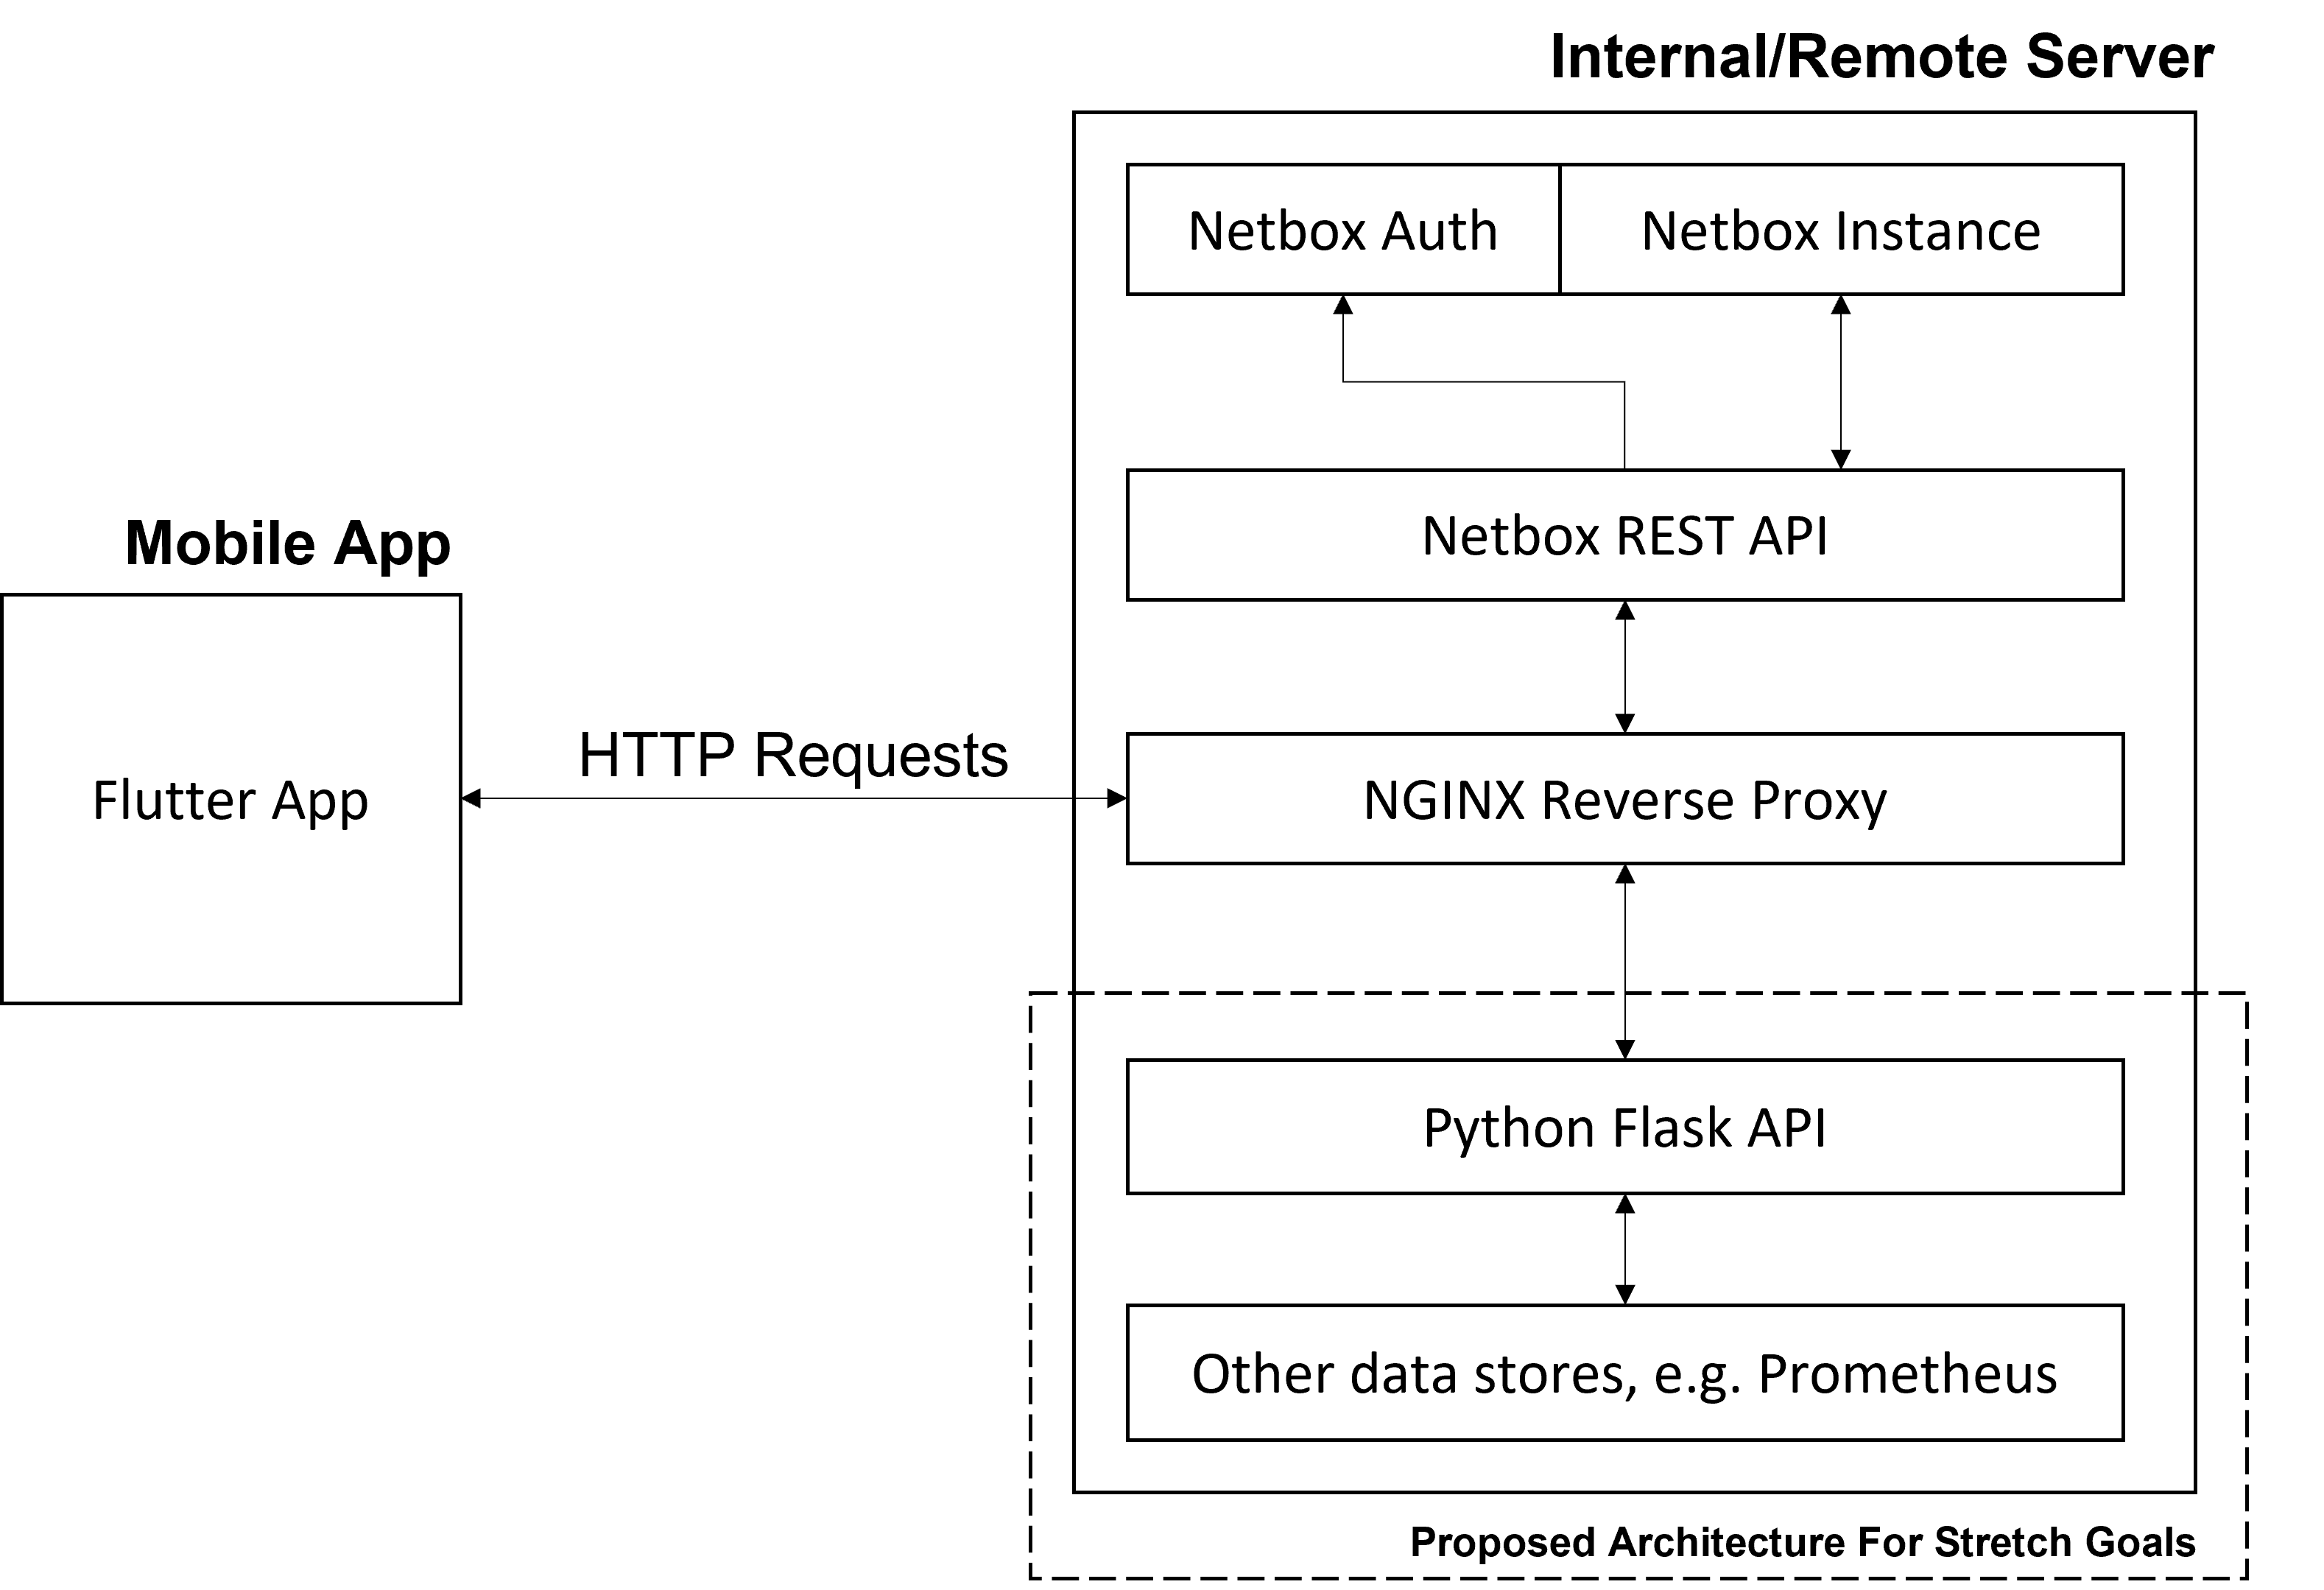
\includegraphics[width=0.6\textwidth]{images/top-level-archi.png}
    \caption{System Architecture}
    \label{fig:architecture}
\end{figure}

The app will use Netbox's inbuilt Django user authentication system, which allows for tokens to be created via an API call. This token will then be used to authenticate the user to fetch data and make changes to the netbox instance, returning any errors should a permission problem arise. For stretch goals, should the app feature more information or processing - The requests will still go through the same NGINX reverse proxy but to a different API endpoint - Though open to change, a Python based Flask Server will be used. 

The app will be structured using a Data Access Object (DAO) pattern\cite{dao}, with the aim of separating the data access from the logic. In a way replicating the data objects within Netbox itself. This will allow for the app to be easily extended and modified in the future. 

Further, there is a separation between views, API calls and providers. This gives a more modular structure and provides more maintainable code, especially as requirements change, or Netbox updates/changes. Additionally, in the spirit of Open Source Software, the code will be stored on Github \cite{keeptrackgithub} and will utilise environment variables to store sensitive information so that other developers can easily implement their own instance of the app.

\subsection{Technical Work Done To Date}
\label{sec:technical_work}
The current technical work has focused on the development on the core logical structure of the app and the creation of a foundation for the UI to test functionality. The current progress allows a user to sign into the app using their Netbox credentials. This information is then stored securely using the Flutter Secure Storage plugin \cite{securestorage}. The current UI allows the user to add a connection between two devices. More specifically, it allows to search for devices via a searchable dropdown, which then dynamically loads its interfaces, with a tab view that allows the user to select the interface on each device. Further, the current implementation has a working integration of the barcode/QR code scanner plugin \cite{barcodeScannerPlugin}. See below for screenshots of the current UI, fig. \ref{fig:currentUIScreenshots}. 

\begin{figure}%
    \centering
    \subfloat[\centering Login Page]{{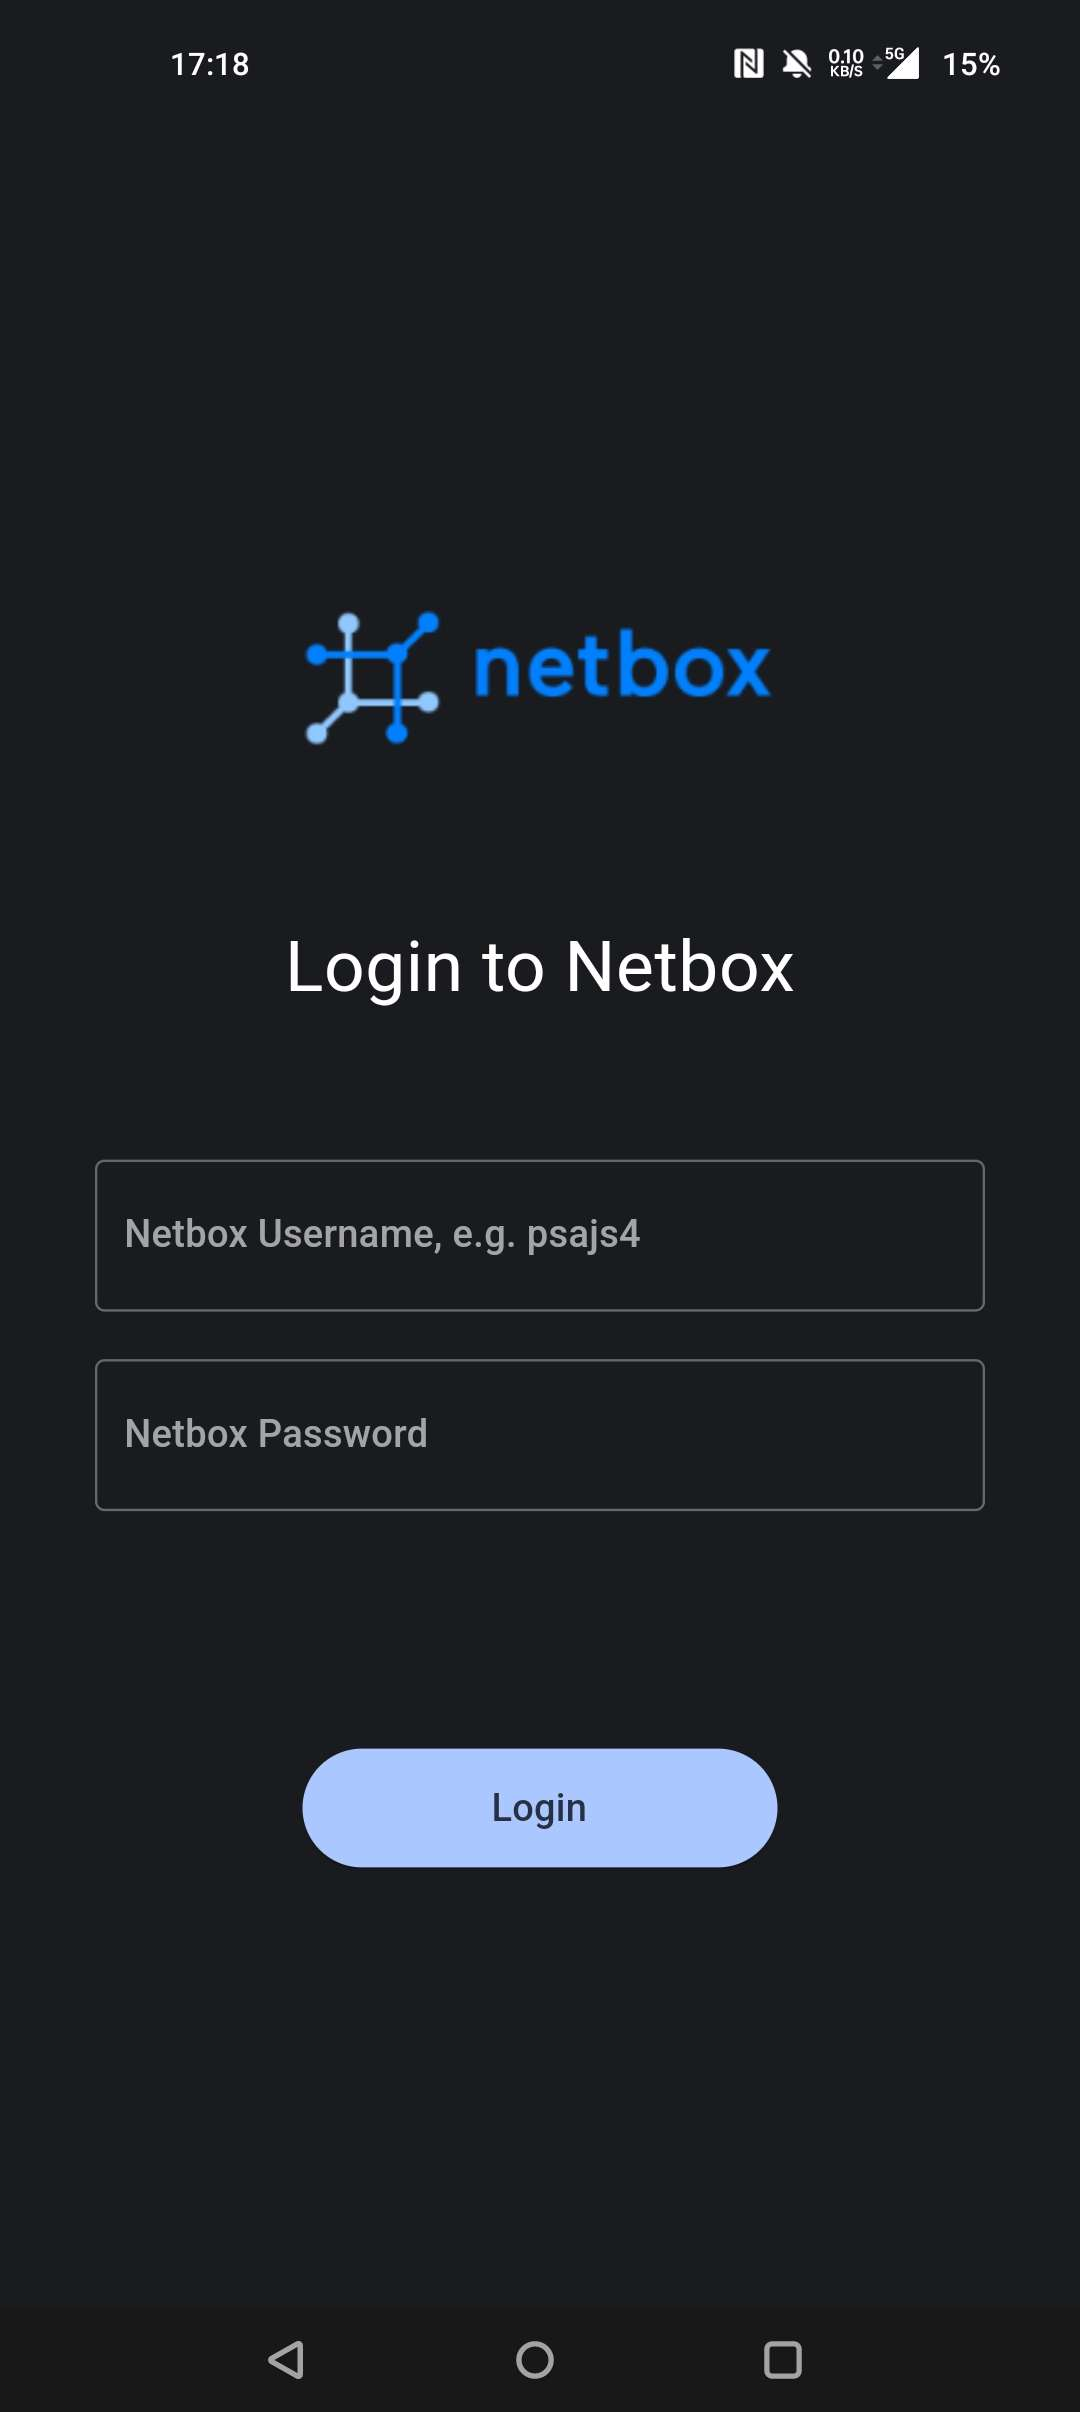
\includegraphics[width=2.5cm]{images/login.png} }}%
    \qquad
    \subfloat[\centering Add Connection Page]{{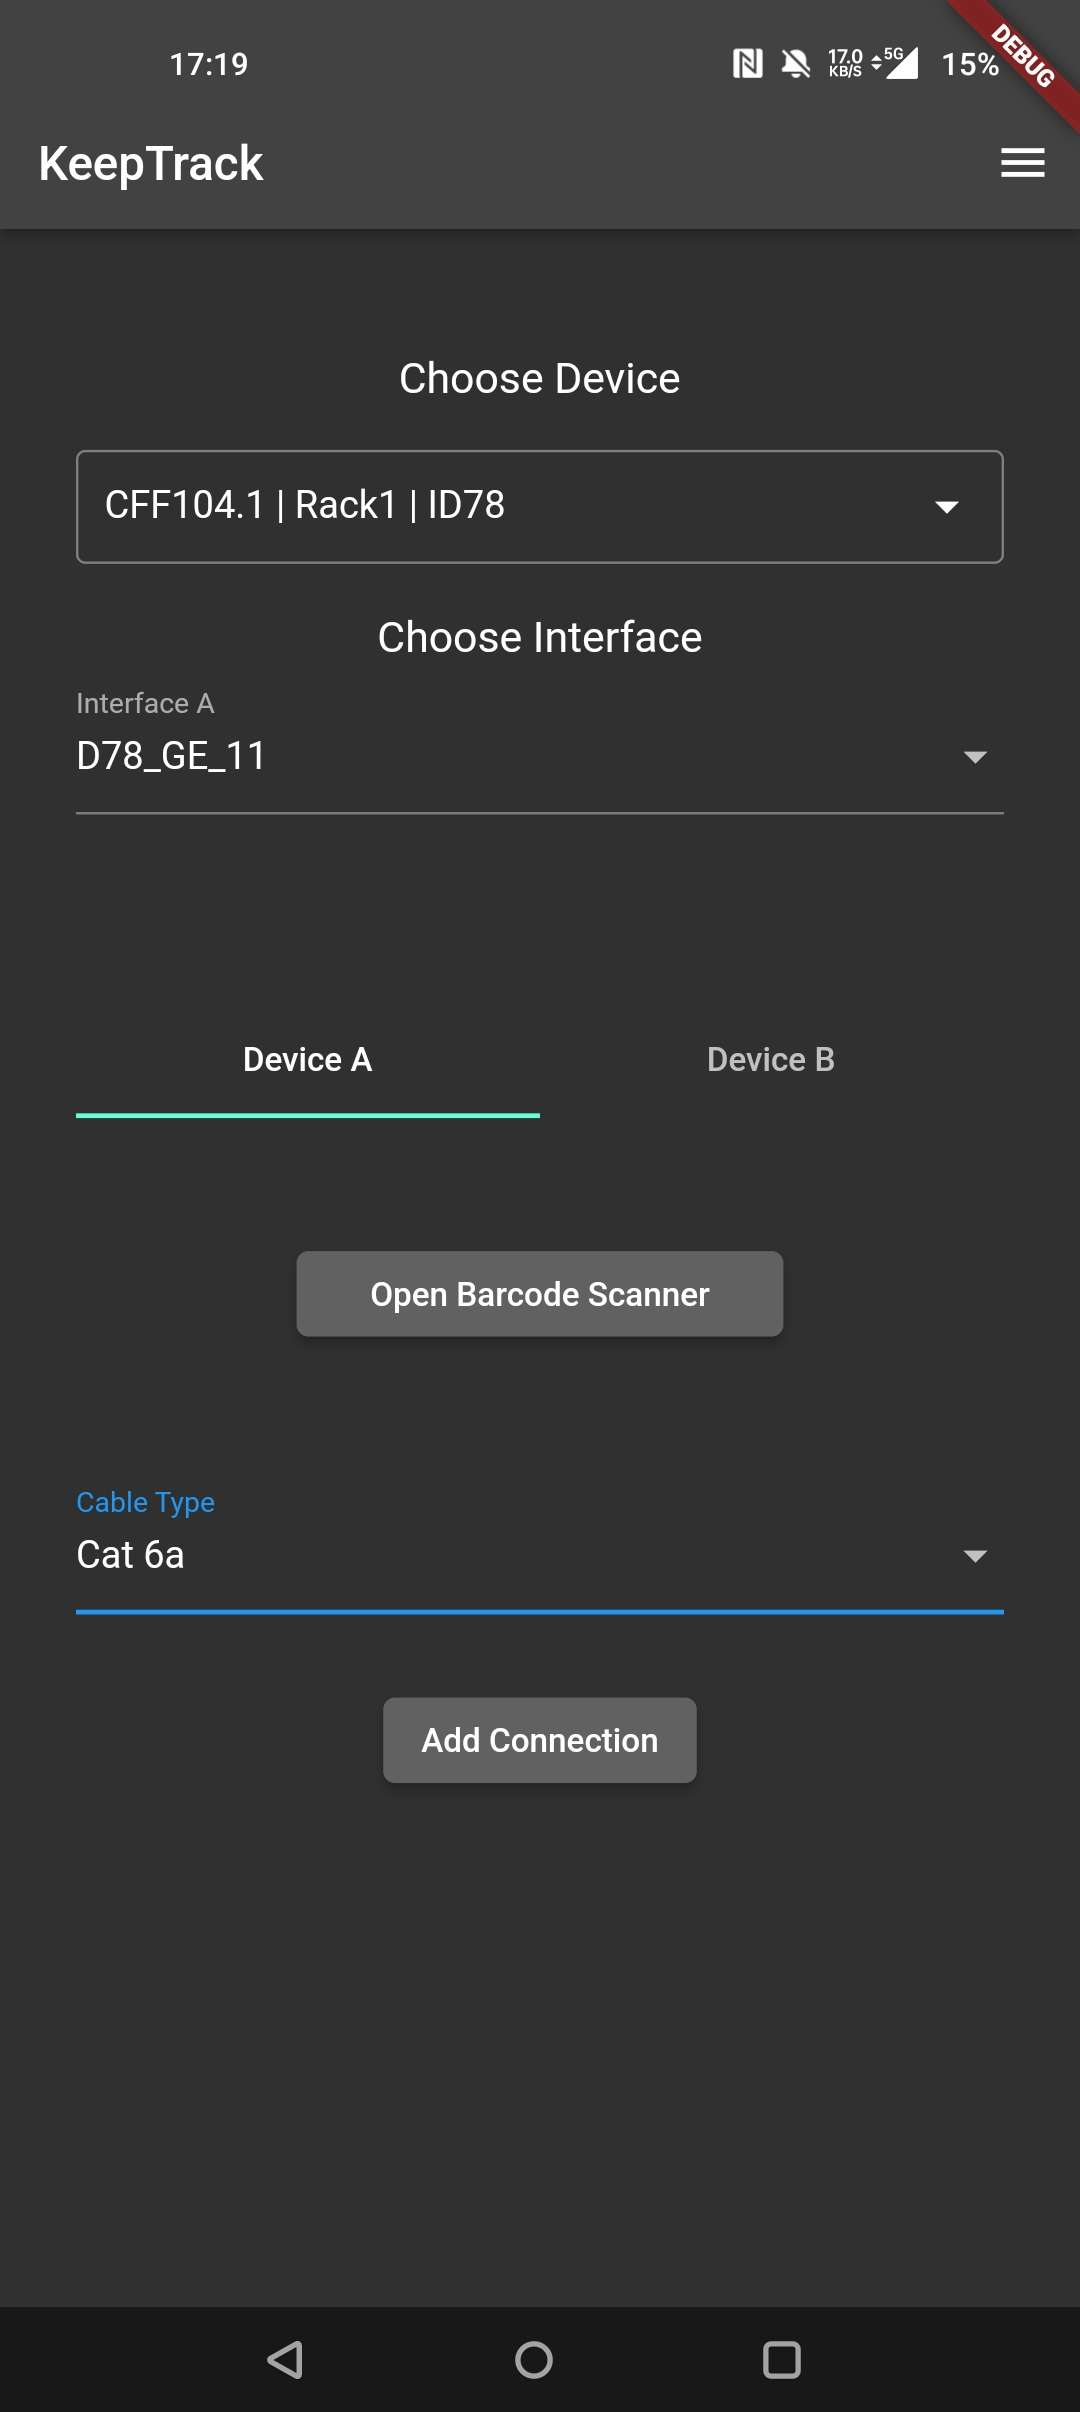
\includegraphics[width=2.5cm]{images/addcon.png} }}%
    \qquad
    \subfloat[\centering Device Search]{{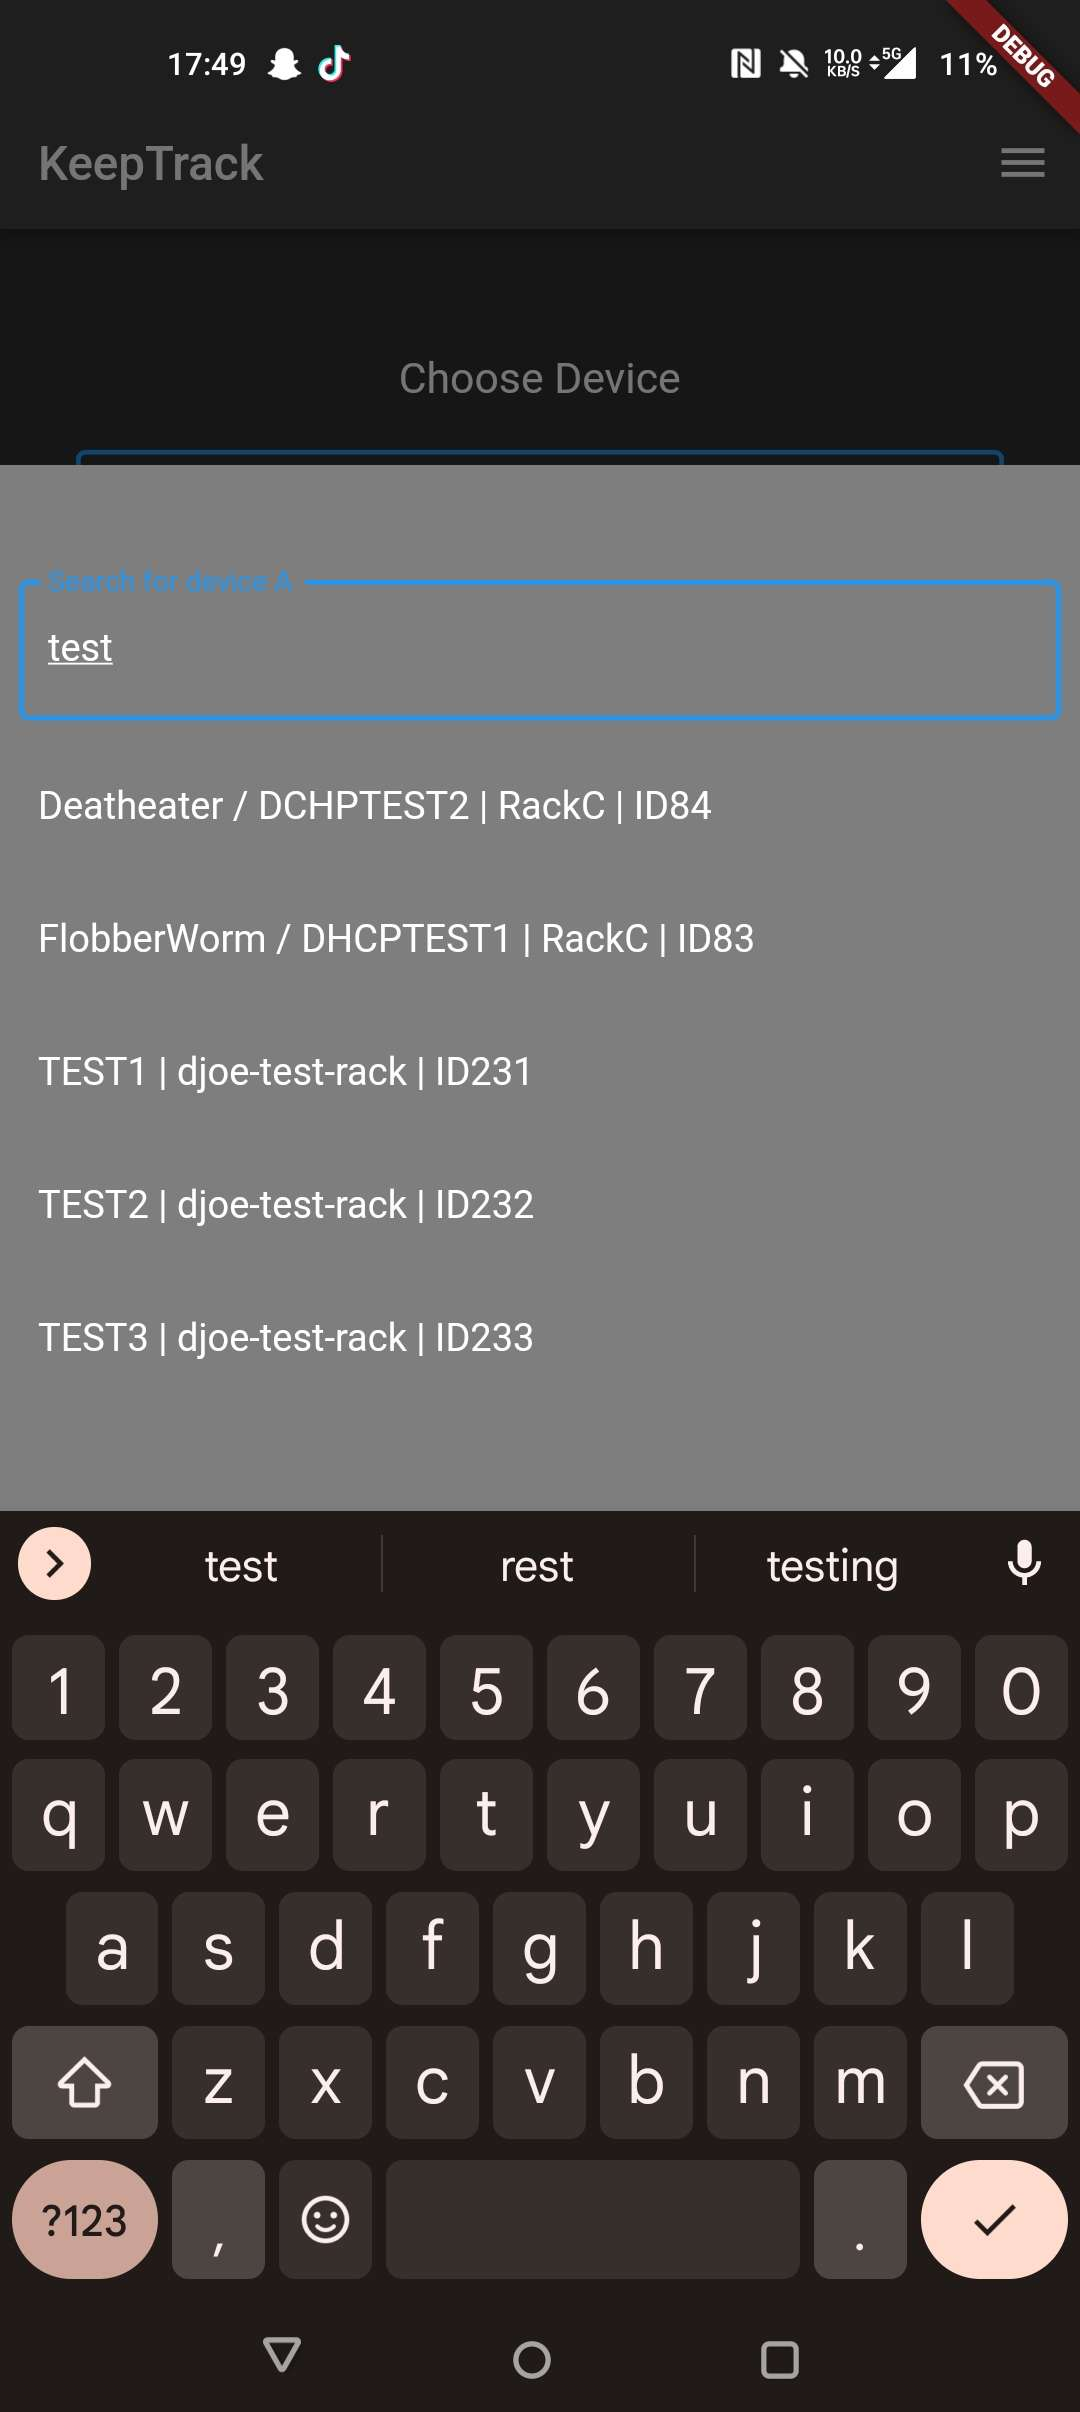
\includegraphics[width=2.5cm]
    {images/search.png} }}%
    \caption{Screenshots of the current Keeptrack UI}%
    \label{fig:currentUIScreenshots}%
\end{figure}


\section{Progress}
\label{sec:progress}
\subsection{Projection Management}
\label{sec:project_management}
Whilst the project is still in its early stages, there has been some good progress made, though less so than initially planned. This is due to a number of factors. Firstly, I hadn't assigned enough time weekly to work on the project, which has led to a slower progress overall. Secondly, I hadn't accounted for the availability of the interviewees, which has led to a delay in the interviews and therefore the creation of the high fidelity prototypes. However, I have been able to make progress on the technical side of the project, which has allowed me to create a foundation for the UI and the core logic of the app. I am satisfied with said technical progress made and I believe that with the core foundations now in place, technical progress can be completed quicker.

I also didn't expect that the literature review would take as long as it did, or more specifically for this project - Finding similar applications along with technical and HCI based papers. Finding applications that had easily accessible trials posed a harder challenge than I had anticipated. But I believe that the similar work I have found has given me a better insight into a mixture of HCI and technical aspects of the project. Though, I struggled to find HCI focused papers that were related to the scenario posed, e.g. encumbered use of a mobile device. 

On a positive note, the interviews brought up some interesting points that I hadn't considered before. For example, an inbuilt SSH terminal, Augmented Reality features, but also increasing the scope of the project to include other rooms. Whilst some of the ideas risen can be achieved easily, others will require more time and research. However, I believe that the interviews have been a success and have given me a better understanding of the stakeholders and their needs.

With the delay to the overall work completed, and a change in some aspects of the project - I have had to re-evaluate aspects of my new work plan. Shifting milestones along and re-assigning tasks to more/less work. I believe I hadn't accounted for a large enough research period, i.e. finding similar work, in the original work plan but now that this has been completed I can focus on getting on with the technical work.

Comparing the initial Gantt chart, fig. \ref{fig:initialworkplan}, to the updated Gantt chart, fig. \ref{fig:updatedworkplan}, it has become apparent that I have had to shift the milestones along. But this mainly filled most of the run over time I had assigned in the initial plan. But even with these delays I am confident that I can complete the project within the time frame given.
\begin{figure}[ht]
    \centering
    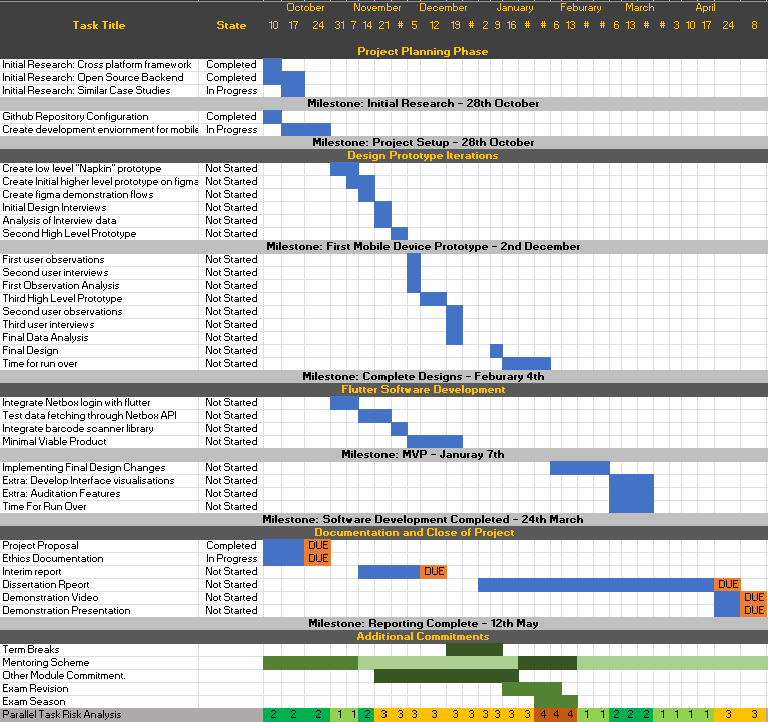
\includegraphics[width=0.8\textwidth]{images/keeptrack-gantt-initial.png}
    \caption{Initial Work Plan/Gantt Chart}
    \label{fig:initialworkplan}
\end{figure}

\begin{figure}[ht]
    \centering
    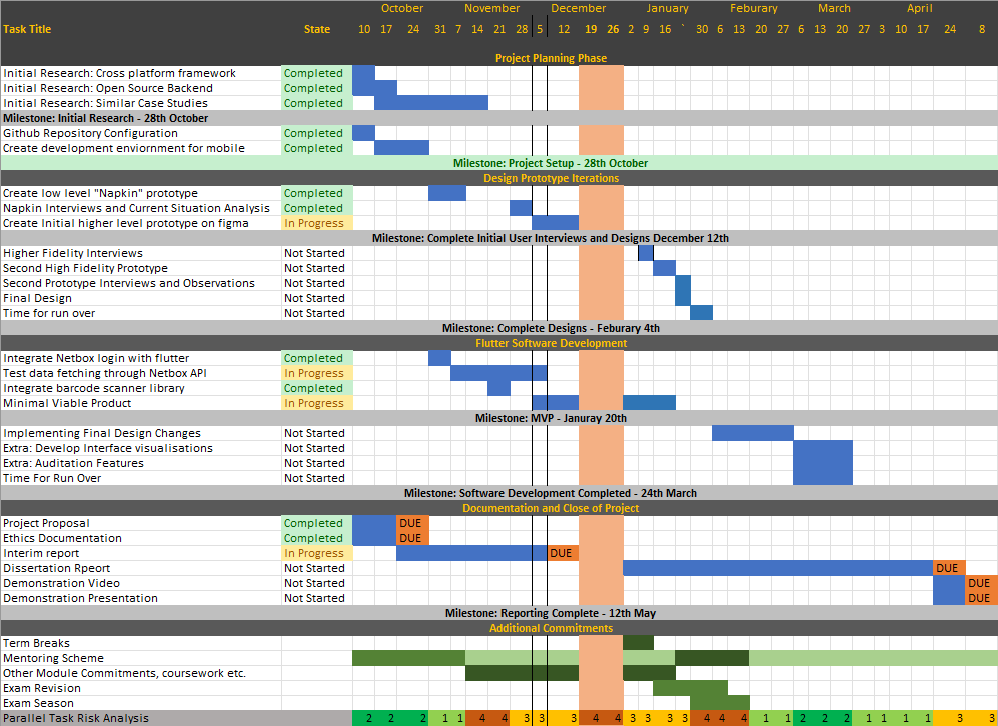
\includegraphics[width=0.75\textwidth]{images/keeptrack-gantt-interim.png}
    \caption{Updated Work Plan/Gantt Chart}
    \label{fig:updatedworkplan}
\end{figure}

During weekly meetings with my supervisor, we have discussed the progress made and the work that needs to be completed. To keep track of the discussions we had I maintained a document. Each meeting I would write up a summary of topics I wanted to discuss, and then during the meeting add notes to each section. Then following the meeting, I would review a Trello board (\ref{sec:trello_board}) to see what tasks I had completed and what tasks I needed to complete. Though initially I didn't assign dates to each task, after falling behind I assigned dates to each task, as well as color coding them based on work type. 

\subsection{Contributions and Reflections}
\label{sec:contributions}
The primary contributions I have made to the project so far is the literature review, interviews and technical work done to date. From this work, I will be able to create a set of high fidelity prototypes and start creating a Minimal Viable Product (MVP) soon after. Though, I am aware that I have somewhat fallen behind on the project. I estimate this to only be a week or two behind, but with the reshuffling of the work plan, and the time set aside for run over, I am confident that I can complete the project within the time frame given.

Overall I am happy with the progress made so far. Initially, whilst I had a good idea of what the app needed to be, following the work done I have a better understanding of what will make the app useful. I have also learnt that there is a significant lacking in the market for a product like this.  I think it to be important that I reach out to external stakeholders, outside of the university, to get a better understanding of the market and what is needed. It is possible that that more ideas will arise from this and that the project will not be limited to what RST needs. 

I think that with the next steps of the project it is important that I establish a more constant workflow, rather than bursts of work I have carried out so far. I think that this will create a more iterative progress and can prompt for more user feedback. Notably, I think that there is a bigger risk of feature creep than I expected and I think I will need to pay more attention to this moving forward.

\subsubsection{Laws, Social, Ethical and Professional Issues}
\label{sec:computer_laws}
As this project intends to be open source under the Mozilla Public License Version 2.0 I foresee no implications of intellectual property. It is currently and will be publicly available via Github \cite{keeptrackgithub}. Though, it is possible the work may be exploited for commercial gain but is dependant on the success of the project and the possibility to be implemented externally.


On the topic of ethics, due to the project involving human participants, I have had to complete the full ethics form, "CS REC 1", and have received approval from relevant parties. Further as set out by the Research ethics guidelines \cite{ethicsguidelines}, I have completed the Data Management Plan (DMP) form. This form outlines how I will store and manage the data collected during the interviews. Each of the interviewees has been given a consent form to sign, which outlines the purpose of the interview and the data collection. The interviewees have also been given the option to opt out of the interview at any point. Additionally, there are notices regarding the Data Protection Act 2018. The data collected will be stored on a password protected computer and will be deleted after the project has been completed.

I believe that on a broader perspective, this project will not have a significant implications on society. Though, I do believe that it will have a positive impact on the RST team and the wider system administrator community. I believe with with the project being open source and with a focus on HCI it will be accessible to a wide range of people. Further by giving DCIM software another platform to be accessed, I believe that this will be a positive step towards the future of DCIM software and data center management.

% Bibliography
\pagebreak
\bibliographystyle{ieeetr}
\bibliography{citation} 

% Appendix
\appendix
\section{Appendix}
\label{sec:appendix}
\subsection{Trello Board}
\label{sec:trello_board}
\begin{figure}[ht]
    \centering
    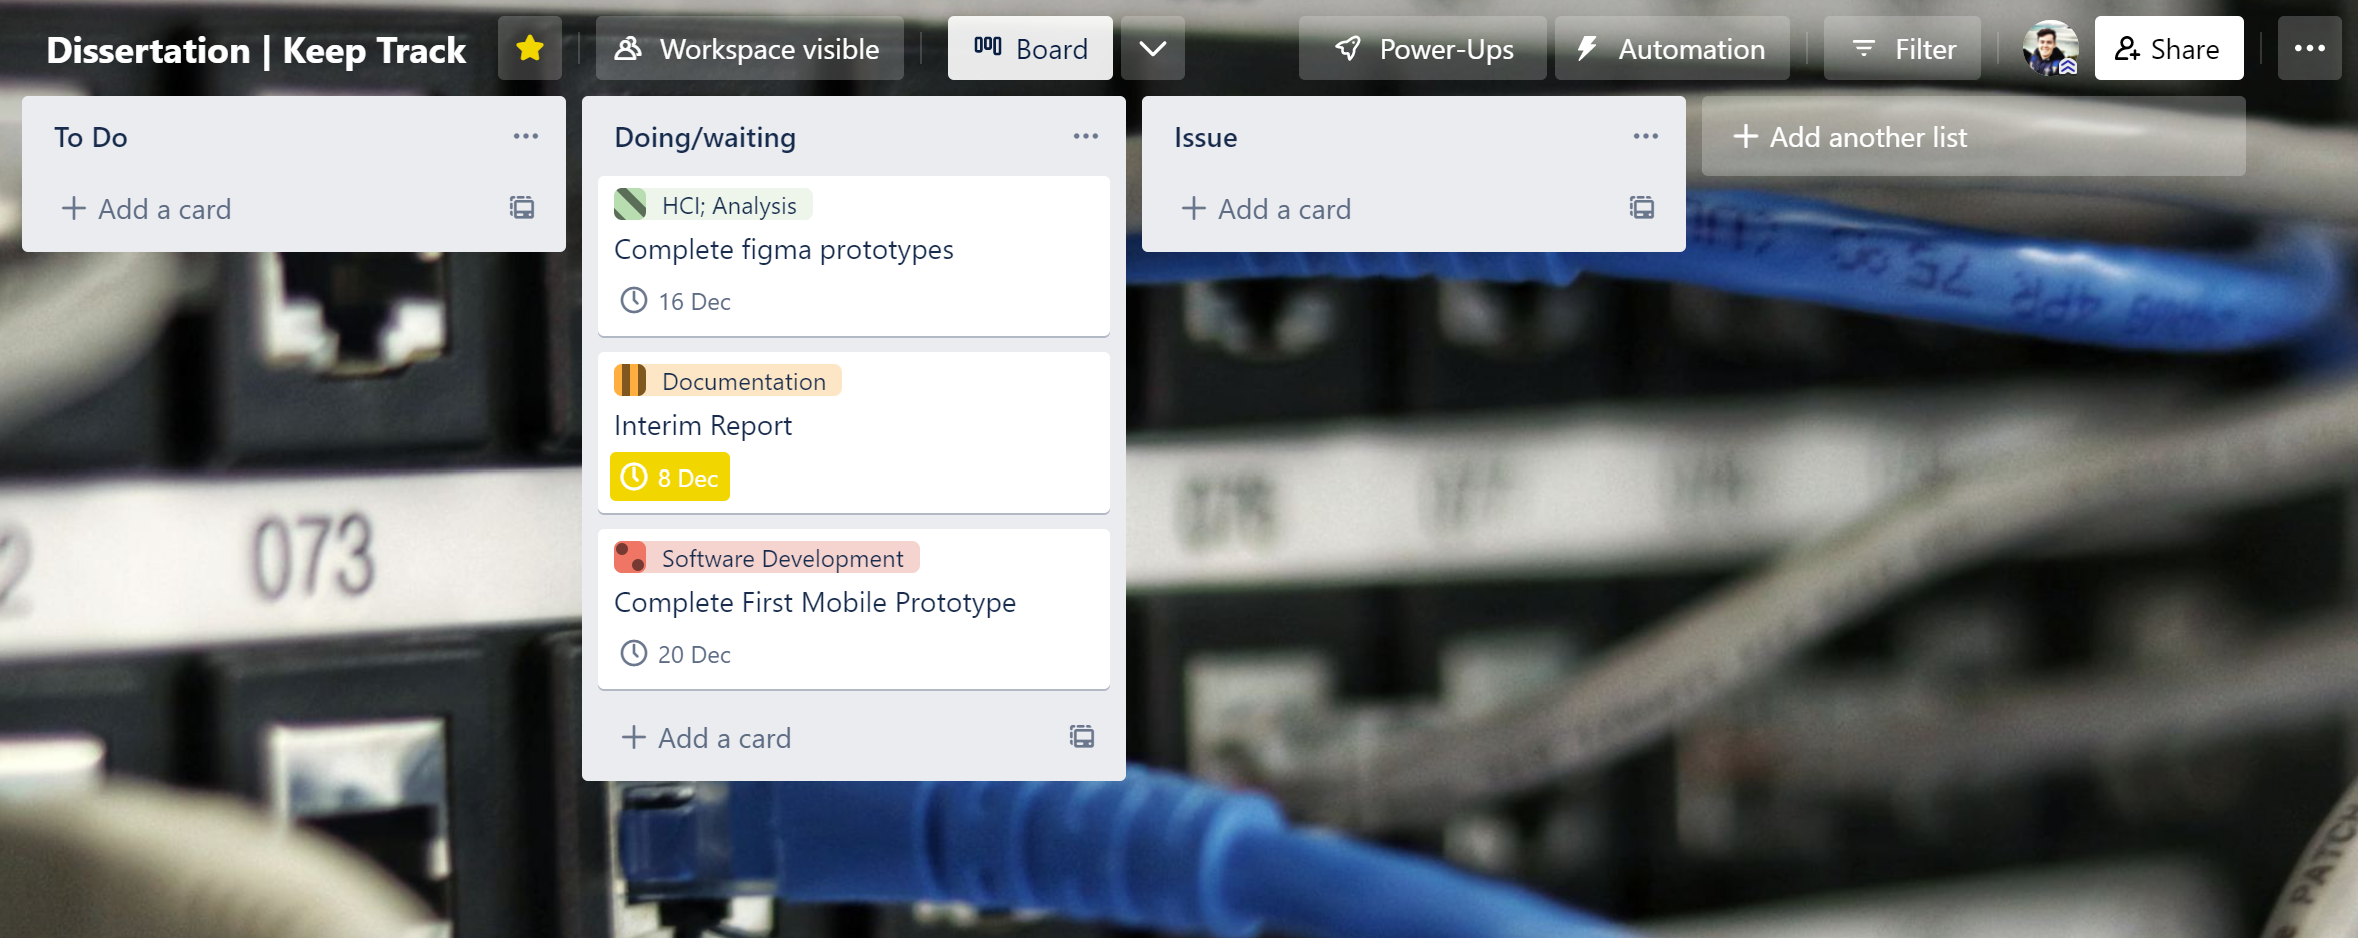
\includegraphics[width=1\textwidth]{images/trello-board.png}
\end{figure}
% Document End
\end{document} 